\chapter{Анализ предметной области}

Изображения и иллюстрации стали использоваться повсеместно --- возникла проблема, связанная с их большим размером. В последние годы решению этой проблемы уделяется достаточно серьезное внимание. Разработано большое количество различных алгоритмов архивации графики: использовались как видоизмененные универсальные, так и абсолютно новые алгоритмы, ориентированные только на изображения. Более того, были разработаны алгоритмы, ориентированные только на конкретный класс изображений.

Для того, чтобы вести речь об изображениях, необходимо определить, что под ними понимается.

\section{Цифровое изображение (Digital Image)}

Цифровое изображение представляет собой изображение, полученное путем оцифровки аналогового изображения с использованием пикселей в качестве основных элементов, и может быть сохранено и обработано цифровым компьютером или цифровой схемой. \cite{DI}

В зависимости от способа описания, изображение может быть растровым или векторным.

\textbf{Растровое изображение} --- изображение, представляющее собой сетку пикселей.

\textbf{Векторное изображение} --- изображение, получающееся путём математического описания элементарных геометрических объектов, обычно называемых примитивами, таких как точки, линии, сплайны, кривые Безье, круги и окружности, многоугольники.  


В данной работе речь пойдет о растровых изображениях.

\section{Сжатие избражния}

Цель сжатия изображения --- уменьшить объем данных, необходимых для представления цифровых изображений. Основным принципом уменьшения объема данных является удаление лишних данных. С математической точки зрения этот процесс фактически преобразует двумерную матрицу пикселей в статистически не связанный набор данных. \cite{10}



%Принцип сжатия изображения.
%\begin{itemize}
%	\item Объектом сжатия данных являются данные, и большой объем данных не означает, что он содержит большой объем информации.
%	\item Сжатие изображения заключается в удалении лишних данных на изображении и не оказывает существенного влияния на информацию.
%	\item Сжатие изображения реализовано в форме кодирования изображения, где меньше битов представляют уровни серого с более высокой вероятностью появления, а большее количество битов представляют уровни серого с более низкой вероятностью появления, так что средняя длина кода ближе к Информационная энтропия.
%\end{itemize}

Задача сжатия изображения состоит из двух основных частей:
кодирование и декодирование. %Если декодированное изображение всегда в
%точности соответствует кодируемому изображению, то такой алгоритм
%кодирования-декодирования называется алгоритмом сжатия без потерь. Если
%декодированное изображение отличается от кодированного, то подобный
%алгоритм называют алгоритмом сжатия с потерями. 
Общая схема процесса
сжатия изображения представлена на рисунке 1.1.

Рассмотрим этапы процедуры сжатия данных в общем виде. Любой метод
сжатия реализует три основных этапа (рис. 1.1):
\begin{itemize}
\item кодирование или первичное сжатие;
\item вторичное сжатие;
\item декодирование или восстановление изображения.
\end{itemize}

На первом этапе выполняется преобразование исходных данных из одной
формы представления в другую. В частности, при сжатии изображений в
зависимости от вида алгоритма сжатия может быть выполнен переход от
исходного изображения (матрица пикселей) к преобразованному изображению (матрица компонент спектра, набор коэффициентов преобразования или описание объектов изображения). \cite{9}
 
На втором этапе компоненты преобразования квантуются и приводятся к
виду удобному для статистического кодирования, а затем кодируются. \cite{10}

%\begin{tabular}{|l|l|}
 % \hline
  %Исходное изображение  & Преобразованное изображение\\
  %\hline
   %& Матрица компонент спектра \\
   %
	%				&( спектральные преобразования) \\ \cline{2-2}

  % Матрица пикселов & Набор коэффициентов преобразования \\
   
	%				&( фрактальное сжатие) \\ \cline{2-2}

   %& Описание объектов изображения \\
   
	%				&( сжатие с распознаванием) \\ 
  %\hline
%\end{tabular}

  \begin{figure}[h!]
    	\centering
    	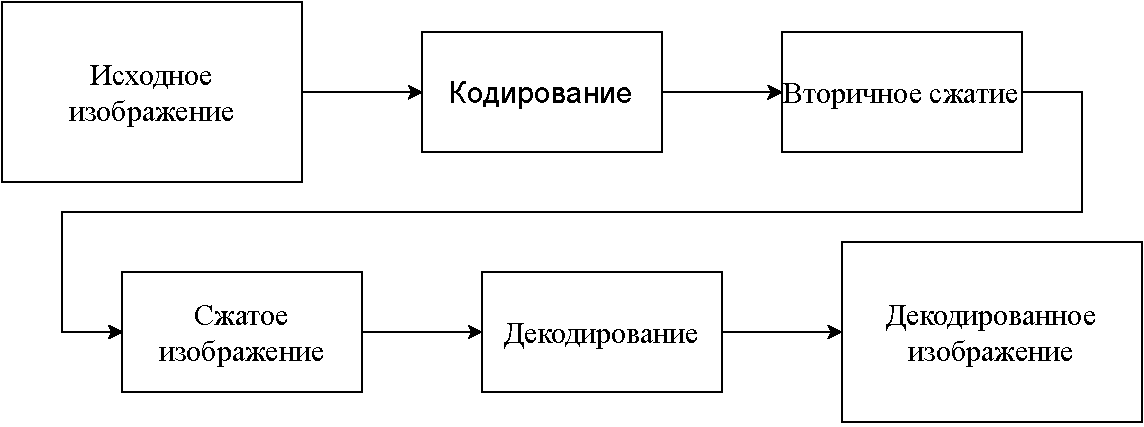
\includegraphics[width=\textwidth,height=10cm,keepaspectratio]{Zip.pdf}
    	\caption{Основные этапы сжатия цифровых изображений} \label{fig:zip}
    \end{figure}
    
   	%RGB (модель является основной при создании и обработке компьютерной графики, предназначенной для электронного воспроизведения ).
        
    %Модель RGB является аддитивной, то есть любой цвет представляется сочетанием в различных пропорциях трех основных цветов --- красного, зеленого, синего.
    
    %\begin{figure}[h!]
    %	\centering
    %	
\includegraphics[width=\textwidth,height=5cm,keepaspectratio]{rgb.png}
    	%\caption{Модель RGB.} \label{fig:rgb}
    %\end{figure}
    
    \newpage
    
    Основная величина, характеризующие метод сжатия --- коэффициент сжатия.
    
    \begin{equation}
    	K_c = \frac{V_1}{V_2},
    \end{equation}
    
    где \(V_1\) --- объем изображения до сжатия, \(V_2\)  --- объем изображения после сжатия.
    
    Этот параметр определяет во сколько раз файл, хранящий сжатое
изображение, меньше файла, хранящего исходное изображение. Величины \(V_1\) и
\(V_2\) выражаются в байтах. \( K_c \) – величина безразмерная.
        
    \section{Вывод}

В данном разделе определены основные термины: цифровое изображение, растровое изображение и векторное изображение. Так же 
рассмотрено понятие --- сжатие изображения.
